\chapter{An\'{a}lisis de Modos Normales para vSGLT}\label{ch:4}

\section{ANM server}
Se estudia el cotransportador vSGLT mediante el servidor ANM (En ingl\'{e}s Anisotropic Network Model server) de la universidad de Pittsburgh \cite{Eyal2015}\footnote{Recurso disponible en \url{http://anm.csb.pitt.edu/cgi-bin/anm2/anm2.cgi}}. El servidor ANM, como su nombre lo indica, es un servidor web que procesa la informaci\'{o}n de entrada del lado del cliente, en este caso, la informaci\'{o}n de entrada ser\'{a} el pdb y los par\'{a}metros de entrada para realizar los c\'{a}lculos del ANM, mientras que del lado del servidor se procesa la informaci\'{o}n suministrada v\'{i}a un c\'{o}digo escrito en C, MATLAB y Fortran que permite calcular los $n$ primeros modos normales, los factores b, las constantes el\'{a}sticas, las correlaciones entre distintas partes de la mol\'{e}cula y permite visualizar los modos de vibraci\'{o}n mediante java o pymol. Tambi\'{e}n es posible descargar el c\'{o}digo fuente desde la p\'{a}gina del servidor.\\

En la figura \ref{fig:flujo} se encuentra un esquema de la entrada y salida de datos.\\
\begin{figure}[h]
 \centering
    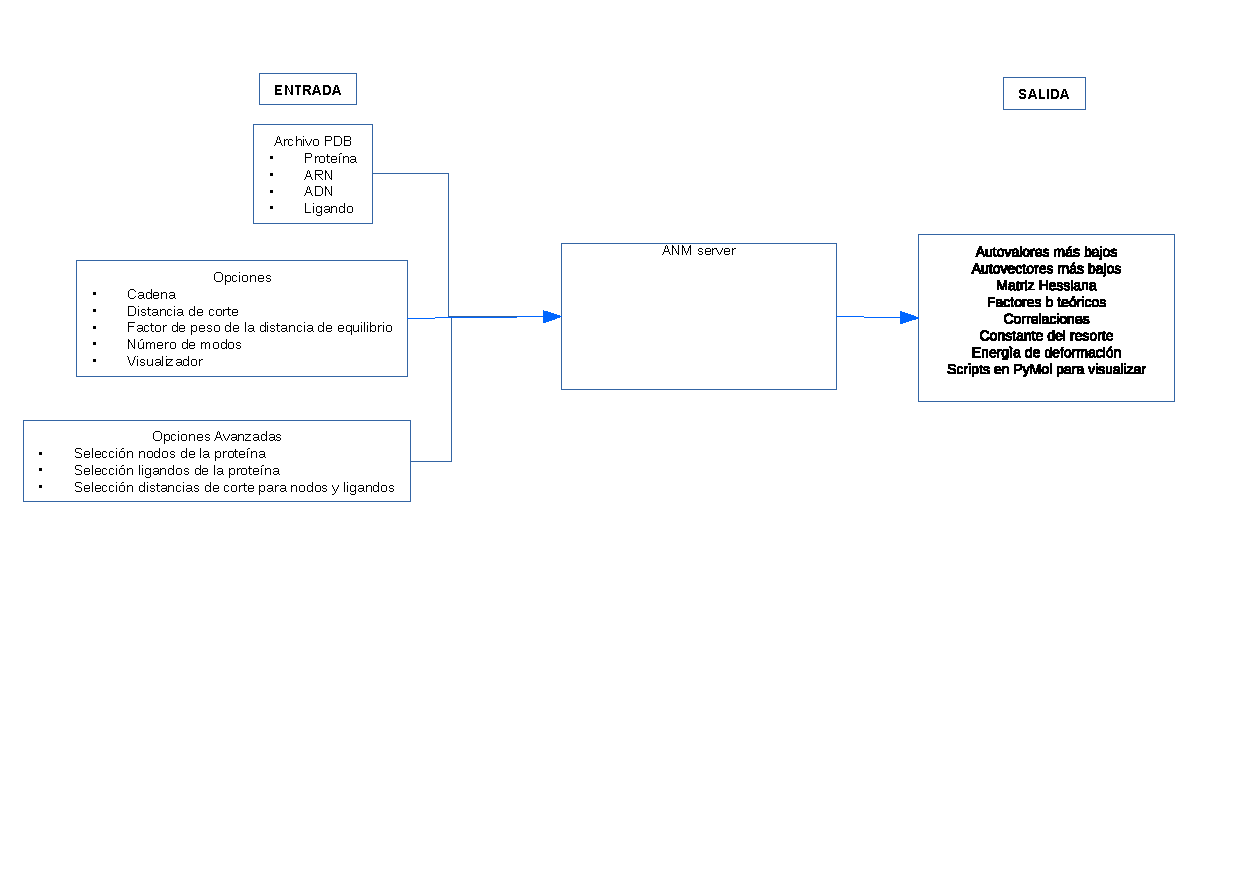
\includegraphics[scale=0.5]{./Kap4/flujo.pdf} 
\caption{Esquema de entrada y salida del servidor ANM}\label{fig:flujo}
\end{figure}
El PDB original se convierte a un modelo en el que se utilizan los carbonos $\alpha$ encontrados en la cadena principal de la prote\'{i}na y si el archivo pdb tiene \'{a}cidos nucl\'{e}icos estos pueden incluidos en el modelo. En el modelo tambi\'{e}n se pueden incluir los ligandos como iones y substratos.\\
\section{NMA previo de vSGLT}
\subsection{Metodolog\'{i}a}
Mediante el servidor ANM, se ha realizado un estudio previo del simportador vSGLT   \cite{Cabrera2017} , en el cual se utiliza el archivo de entrada 3dh4.pdb \cite{Faham2008} encontrado en la base de datos del PDB como tetr\'{a}mero. En este archivo pdb no se determinan los residuos de la primera h\'{e}lice en cada subunidad. Aunque aparecen las posiciones de los residuos, el ANM server los ignora, haciendo el c\'{a}lculo \'{u}nicamente a partir del residuo 47.\\

Una vez ingresado el archivo pdb se selecciona el modelo de la estructura. Inicialmente se toman s\'{o}lamente los carbonos $\alpha$ del co-transportador, se seleccionan las distancias de corte $R_c$ entre $7\AA$ y $14\AA$. Adem\'{a}s, el factor de peso aplicado a las distancias de corte es $s=0$, es decir, las distancias de corte en el hessiano \eqref{eq:hes} son fijas \cite{Zimmermann2011}. Luego se calculan los modos normales $(\lambda_k,a_k)$ (autovalores, autovectores) y los factores b mediante la parte del c\'{o}digo escrita en Fortran. Se hace otro NMA agregando los \'{a}tomos de la galactosa (sin hidr\'{o}genos), agregando el sodio y luego agregando tanto el ion como el sustrato.\\
\begin{figure}[h]
 \centering
    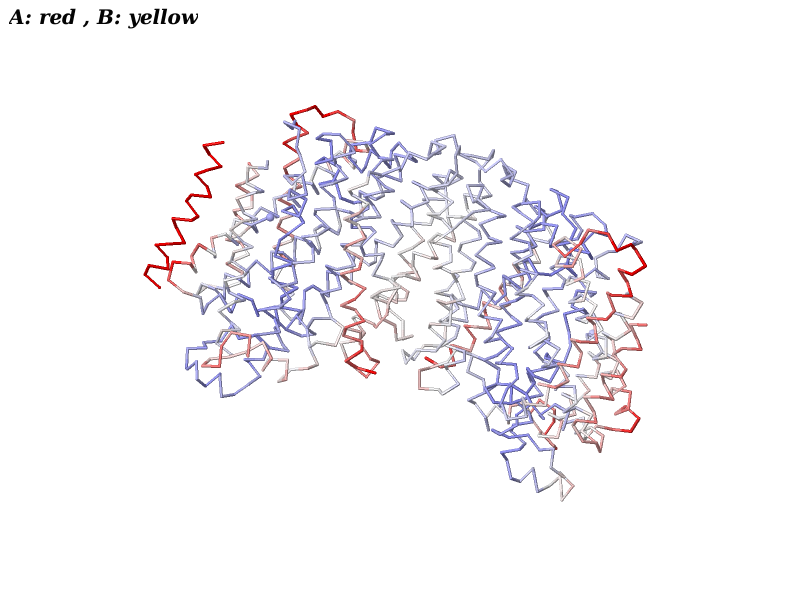
\includegraphics[scale=0.2]{./Kap4/Ca_8_Na_8.png}
    \put(-28,-4){(a)}
    \includegraphics[scale=0.2]{./Kap4/Ca_15_Na_15.png} 
    \put(-28,-4){(b)}
   \caption{Modelo de grano grueso de vSGLT mostrando (a) la cadena principal con los carbonos $\alpha$ conectados por enlaces pept\'{i}dicos. (b) los \'{a}tomos de carbono y el ion de sodio conectados mediante resortes a una distancia de corte de $15\AA$. Imagenes obtenidas con el ANM server \cite{Zimmermann2011}.}\label{fig:modelo}
\end{figure}
\subsection{Resultados}
En la figuras \ref{fig:ANM_pre1}, \ref{fig:ANM_pre2}, \ref{fig:ANM_pre3} y \ref{fig:ANM_pre4} se muestran los factores b por cada n\'{u}mero de residuo (entre 47 y 545) y para cada distancia de corte $R_c$, entre $8\AA$ y $14\AA$ de la cadena A. Ha de notarse que para distancias de corte menores o iguales a $7\AA$,no se encontraron todos  los autovalores, ni autovectores, ni factores b, ya que no todos los autovalores convergen \cite{Zimmermann2011}.\\

En todas las distancias de corte se encontraron 5 picos alrededor de los residuos  S209, M318, T343, I386 y W543 . Exceptuando T343, sus factores B est\'{a} en la tabla \ref{tab:flu2} del anexo \ref{AnexoB}). S209 est\'{a} al final del segmento TM6, M318 est\'{a} al final del segmento TM8 (Este lugar queda en el citoplasma y es donde se dobla TM8), T343 en una peque\~{n}a h\'{e}lice encontrada entre TM8 y TM9, I386 en la regi\'{o}n desordenada entre TM9 y TM10 (en el periplasma) y W543 al final de la cadena A.\\
\subsubsection{Distancias de corte $R_c=8\AA$ y $R_c=9\AA$}

\begin{figure}[ht]
 \centering
 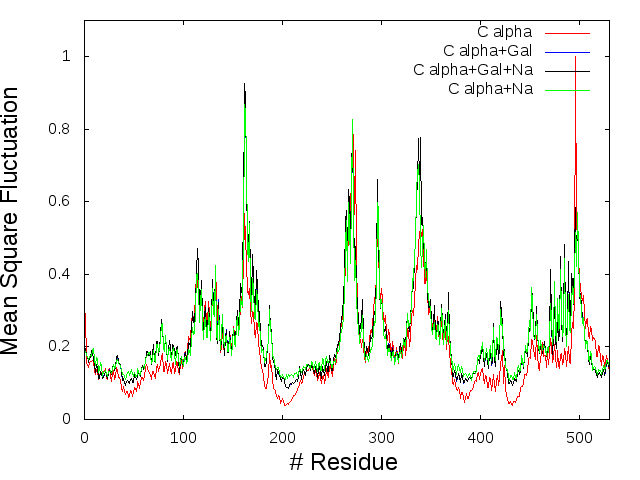
\includegraphics[scale=0.35]{./Kap4/ANM/ANM_server/grafica_8_A_n.png}
  \put(-28,-4){(a) $R_c=8\AA$}
   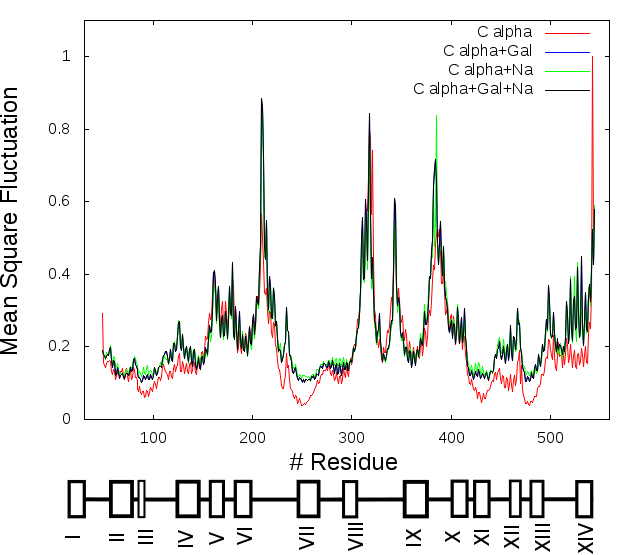
\includegraphics[scale=0.35]{./Kap4/ANM/ANM_server/grafica_9_A_n.png}
  \put(-28,-4){(b) $R_c=9\AA$}
\caption{Fluctuaciones ms normalizadas en funci\'{o}n del n\'{u}mero de residuo para $ R_c=8\AA$ y $R_c= 9\AA$ usando  los primeros 100 modos. Los diferentes colores indican si la simulaci\'{o}n fue realizada sin el ion, el sustrato, con alguno de ellos o ambos.}\label{fig:ANM_pre1}
\end{figure}

Para distancias de corte entre $8\AA$ y $9\AA$, se observa en las gr\'{a}ficas \ref{fig:ANM_pre1} (a) y (b) que la prote\'{i}na  es menos flexible cuando est\'{a} sin unirse a los sustratos (color rojo) desde el segmento TM2 hasta el final del segmento TM14. La excepci\'{o}n es el pico presente en el residuo W543 (Cuyo factor b est\'{a} en tabla \ref{tab:flu2} del anexo \ref{AnexoB}) que presenta mucha m\'{a}s flexibilidad. Esto se debe a que el segmento TM14 est\'{a} lejos tanto del sitio activo de la prote\'{i}na como de la segunda subunidad como se observa en la figura \ref{fig:complejo} donde TM14 es la $\alpha$ h\'{e}lice de color rojo.\\

Los picos correspondientes a los residuos S209 y F210 tambi\'{e}n muestran cambios significativos de la fluctuaciones ms antes y despu\'{e}s de unirse alguno de los sustratos. Estos picos corresponden al comienzo del lazo $\omega$ comprendido entre las segmentos TM6 y TM7.\\

El co-transportador es m\'{a}s flexible cuando al menos uno de los sustratos se encuentra unido a este. Pero los movimientos globales de simportador no difieren significativamente cuando el ion, el soluto o ambos est\'{a}n unidos. Esto podr\'{i}a sugerir que el \ce{Na^{+}} y la galactosa no son de alta cooperaci\'{o}n.\\

Para comprobar esta afirmaci\'{o}n se hace una mirada detallada a las regiones alrededor de los residuos Ile253, Glu88, Phe479, Ile438 y la regi\'{o}n con los residuos Glu384,Tyr385 y Ile386.\\

Los residuos Glu384, Tyr385 y Ile386 corresponden a la regi\'{o}n desordenada comprendida entre los segmentos TM9 y TM10, que como se espera, es m\'{a}s flexible que las $\alpha$ h\'{e}lices y por esta raz\'{o}n los cambios en los movimientos son mayores .\\

M\'{a}s interesante es el segmento TM7, donde se encuentra Ile253. Esta regi\'{o}n es m\'{a}s r\'{i}gida cuando el cotransportador est\'{a} libre (color rojo) teniendo la conformaci\'{o}n ocluida. Cuando se une el \ce{Na^{+}}, TM7 se vuelve $\sim 3$ veces m\'{a}s flexible (color verde) pero cuando se une tanto el sodio como la galactosa TM7 se vuelve m\'{a}s r\'{i}gido.\\

En la figura \ref{fig:Gal_h7} se muestra como cambia la flexibilidad del segmento TM7 cuando el cotransportador s\'{o}lo tiene los C-$\alpha$ y cuando est\'{a} con unido tanto al \ce{Na^{+}} como a la galactosa. El color azul oscuro indica que inicialmente el segmento TM7 de vSGLT era menos flexible pero posteriormente TM7 se volvi\'{o} m\'{a}s flexible.\\
\begin{figure}[h]
 \centering
    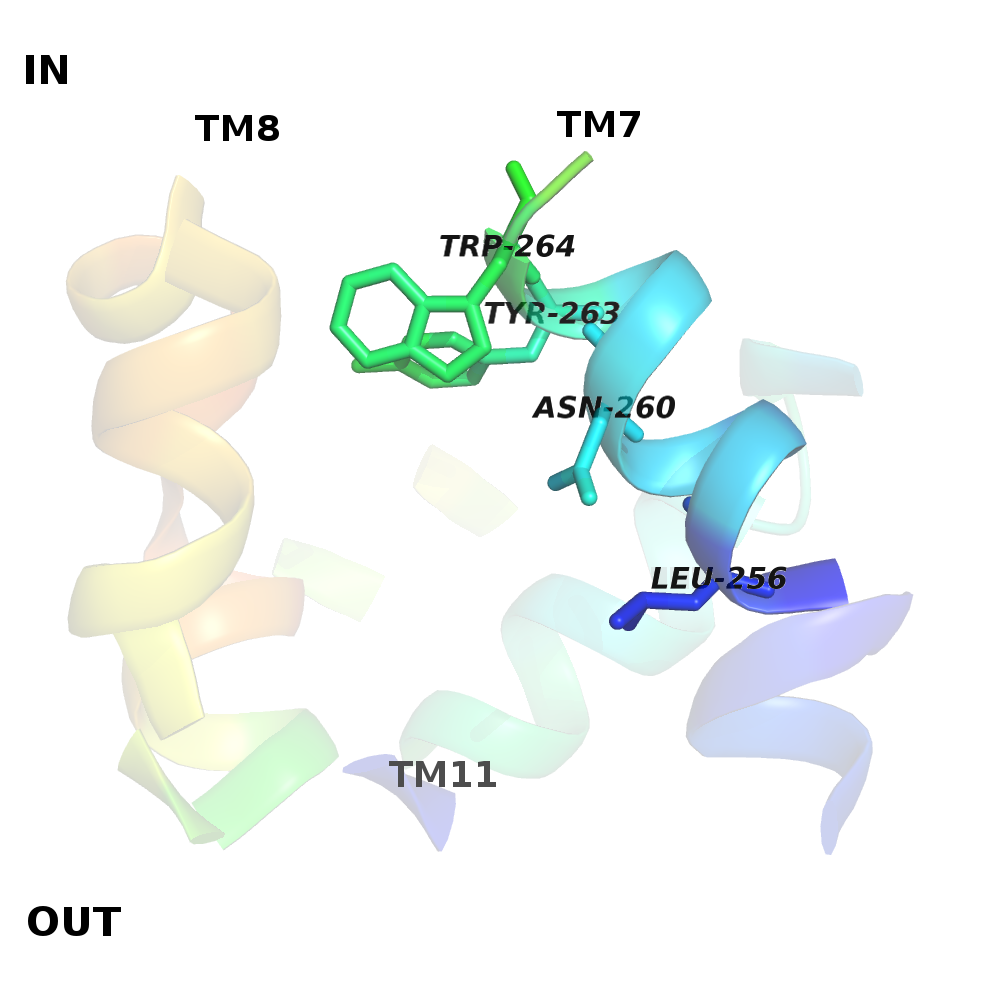
\includegraphics[scale=0.18]{./Kap4/h7_label.png}
    \put(-28,-4){(a) S\'{o}lo C$\alpha$}
    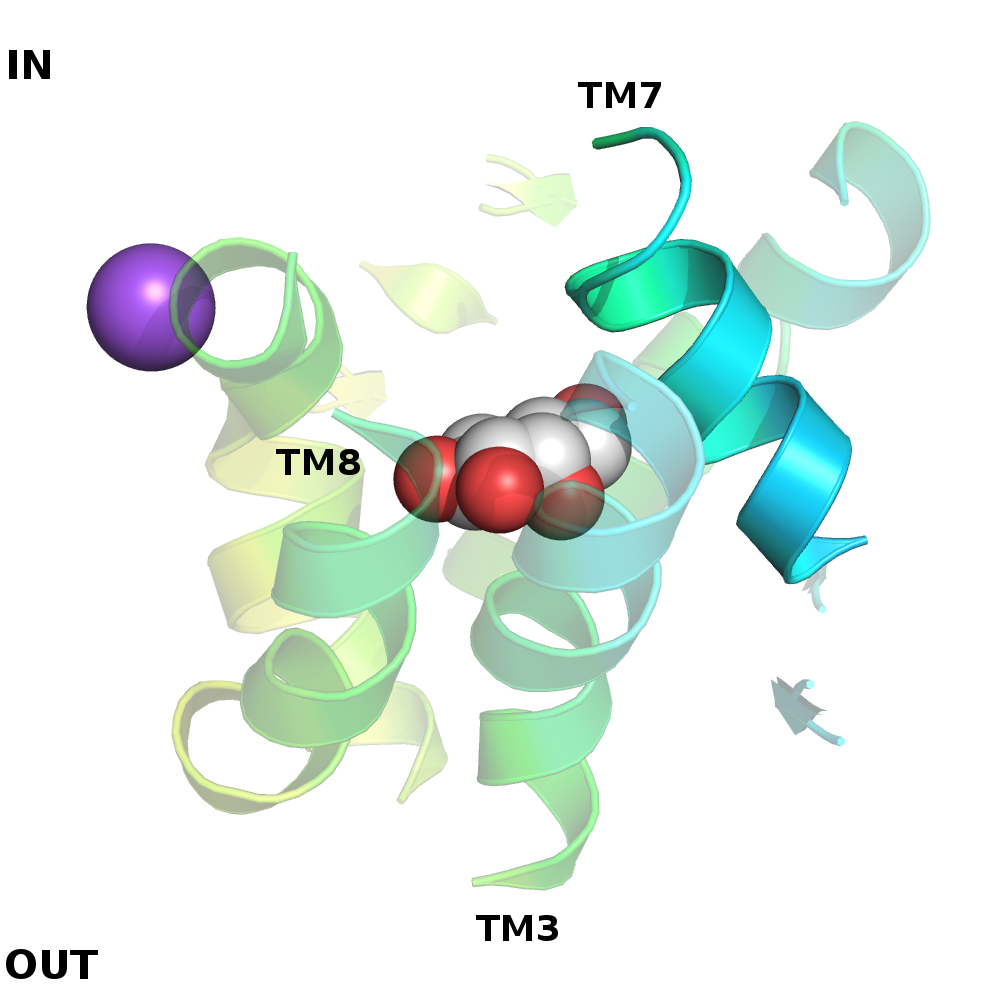
\includegraphics[scale=0.18]{./Kap4/h7_2_label.png}
   \put(-28,-4){(b) C$\alpha+$Na$+$Gal}
\caption{Sitio activo de la galactosa mostrando las $\alpha$ h\'{e}lices involucradas hasta una distancia de $12\AA$. Los colores representan los factores B donde Morado$<$Azul$<$Verde$<$Amarillo$<$Naranja$<$Rojo. El segmento TM7 es m\'{a}s r\'{i}gido pero presenta mayores cambios. En (a) no se muestra el segmento TM3. Imagenes obtenidas con PyMol.}\label{fig:Gal_h7}
\end{figure}

Tambi\'{e}n se observa que la galactosa est\'{a} rodeada por los segmentos Tyr263, Trp264 y Asn260.Se observa que Tyr263 y Trp264 son m\'{a}s flexibles, indicando que de acuerdo a la literatura (en especial Tyr263), act\'{u}an como una compuerta que permite el paso de la galactosa,  ver figura \ref{fig:exit}.\\

La regi\'{o}n en la que se encuentra Glu88 es el segmento TM3, el cual se encuentra en contacto directo con la galactosa. Los cambios en los movimientos en esa regi\'{o}n se deben a la presencia de la galactosa.\\
\subsubsection{Distancia de corte $R_c=10\AA$}

La distancia de corte de $R_c=10\AA$ es una distancia interesante ya que es la distancia aproximada a la que se encuentran el ion de \ce{Na^{+}} y la galactosa.\\
\begin{figure}[h]
 \centering
    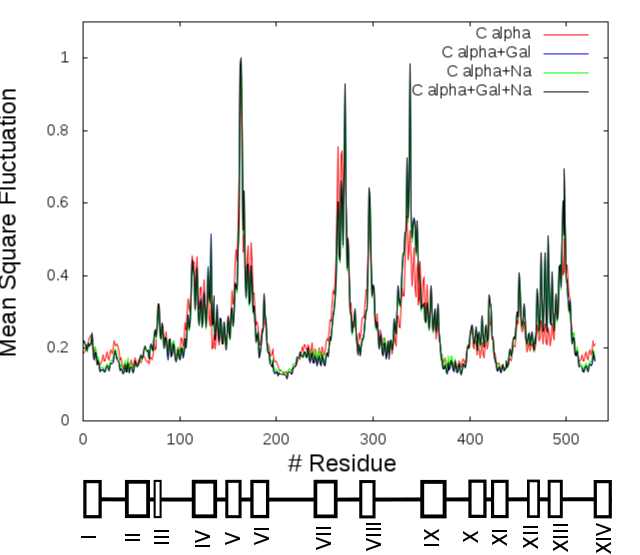
\includegraphics[scale=0.35]{./Kap4/ANM/ANM_server/grafica_10_A_n.png}
   \put(-28,-4){(a)$R_c=10\AA$}
\caption{Fluctuaciones ms normalizadas en funci\'{o}n del n\'{u}mero de residuo para $ R_c=10\AA$ usando  los primeros 100 modos. Los diferentes colores indican si la simulaci\'{o}n fue realizada sin el ion, el sustrato, con alguno de ellos o ambos.}\label{fig:ANM_pre2}
\end{figure}

Contrario a las  primeras dos gr\'{a}ficas, en la figura \ref{fig:ANM_pre2} no se ve una tendencia general de disminuci\'{o}n o aumento de las fluctuaciones ms de la cadena sola (color rojo) o de la cadena con el ion y/o el sustrato unidos. Tampoco se ve una diferencia significativa entre las fluctuaciones cuando \'{u}nicamente la galactosa est\'{a} unida (azul) y tanto el \ce{Na^{+}} y la galactosa est\'{a}n unidas (negra).\\

Hay regiones en las que las fluctuaciones ms aumentan entre el final de segmento TM9 hasta TM10, en el segmento TM12, en el segmento TM14. Las regiones en las que m\'{a}s disminuye est\'{a}n en el segmento TM2, el segmento TM5, en el segmento TM7 y el pico de la regi\'{o}n desordenada desde TM8 hasta TM9.\\

Al comparar la figura \ref{fig:ANM_pre1} con la figura \ref{fig:ANM_pre2} hay una disminuci\'{o}n en la amplitud de las fluctuaciones al final de la cadena, es decir, en el residuo W543. Al observar esta regi\'{o}n que se muestra en la figura \ref{fig:W543} (b), se encuentra que el residuo W543 es estabilizado por los residuos adyacentes, los cuales pertenecen a $\alpha$ h\'{e}lices ubicadas entre los segmentos TM6 y TM7. Sin embargo, estos no forman interacciones electrost\'{a}ticas con el residuo W543 debido a que este es un residuo arom\'{a}tico no polar y a que la parte de su cadena principal est\'{a} a m\'{a}s de $3\AA$ de otras cadenas.\\
\begin{figure}[h]
 \centering
 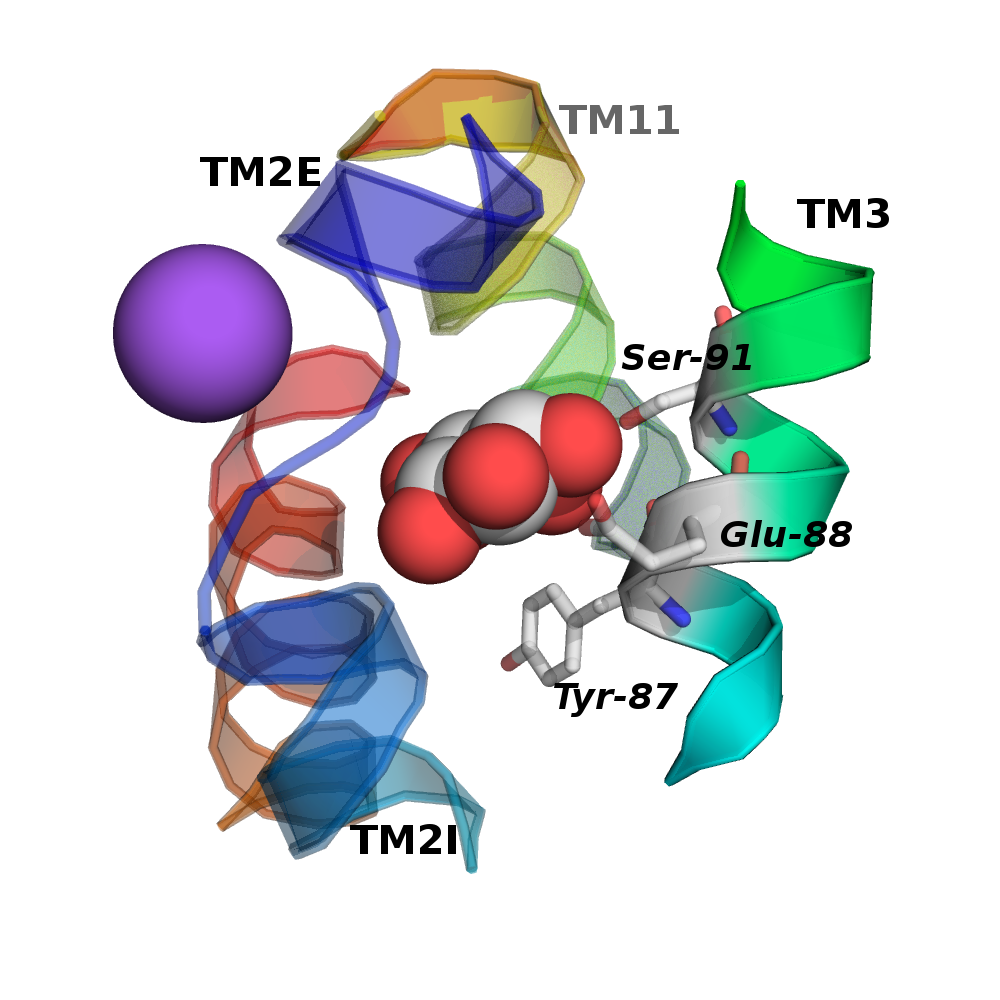
\includegraphics[scale=0.18]{Kap4/h3_h2_label_l.png}
 \put(-28,-4){(a)TM3}
 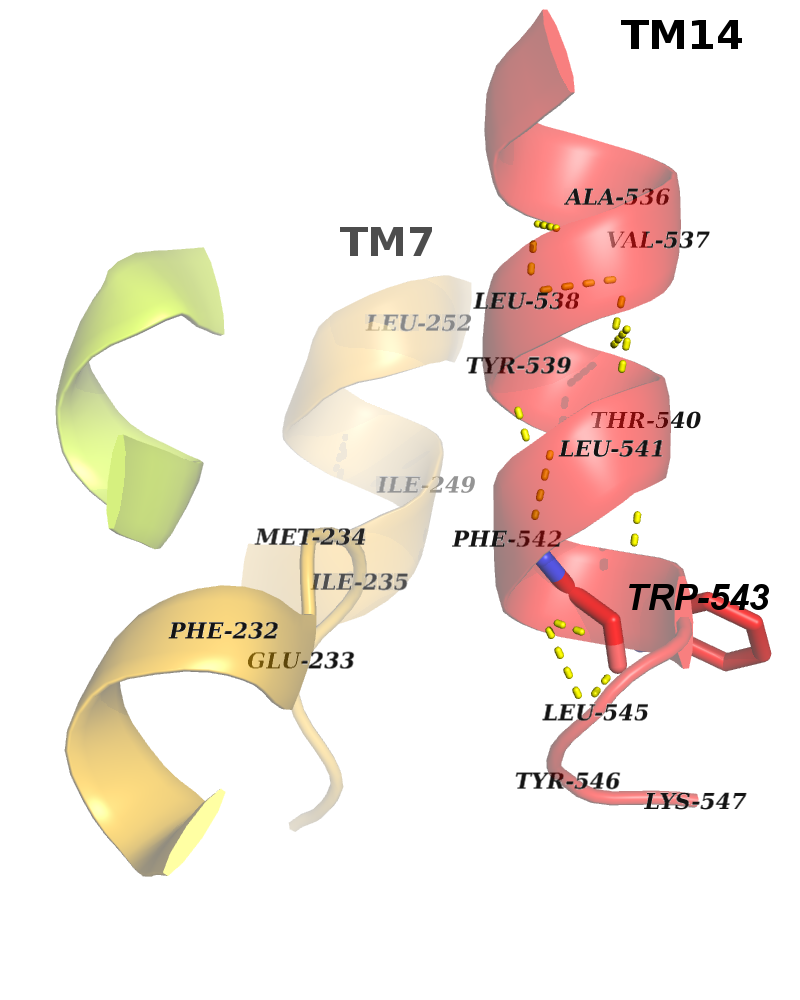
\includegraphics[scale=0.18]{Kap4/W543_label.png}
 \put(-28,-4){(b)TM14}
 % W543_label.png: 0x0 pixel, 300dpi, 0.00x0.00 cm, bb=
 \caption{(a) Contactos entre la galactosa y el segmento TM3. (b)Contactos del residuo W543 a $10\AA$. No se observan interacciones de este residuo con sus vecinos. Imagen y puentes de hidr\'{o}geno obtenidos mediante PyMol.}
 \label{fig:W543}
\end{figure}
Para analizar la cooperaci\'{o}n entre el ion \ce{Na^{+}} se analizan los lugares donde las fluctuaciones son m\'{a}s bajas pero ocurren cambios ligeramente mayores que en el resto del cotransportador, estas son entre TM3 y TM4, TM8 y TM11. Sin embargo, TM8 est\'{a} a m\'{a}s de $10\AA$ de la galactosa (exceptuando por el residuo P263 que  dobla ligeramente la gran $\alpha$ h\'{e}lice de TM8).\\

El segmento TM3 es el que se encuentra m\'{a}s cercano a la galactosa (figura \ref{fig:W543} (a)) por lo que los efectos de la galactosa deben notarse en las distancias de corte $R_c=8\AA$, $R_c=9\AA$ y $R_c=10\AA$. En efecto, al observar las fluctuaciones ms de las gr\'{a}ficas \ref{fig:ANM_pre1} se encuentra un mayor cambio en las fluctuaciones antes (gr\'{a}fica roja) y despu\'{e}s de unirse el \ce{Na^{+}} y la galactosa (gr\'{a}fica negra) y para la distancia de $R_c=10\AA$ se encuentran cambios del orden del $\sim 1\%$. Tambi\'{e}n se observa que hay un cambio cuando solo se une el s\'{o}lo el \ce{Na^{+}} (gr\'{a}fica verde) y cuando se unen el \ce{Na^{+}} y la galactosa (gr\'{a}fica negra). Esto indica que el sodio vuelve la regi\'{o}n m\'{a}s flexible, entreg\'{a}ndole energ\'{i}a, mientras que al unir la galactosa esta regi\'{o}n se vuelve m\'{a}s est\'{a}tica, cediendo energ\'{i}a cin\'{e}tica.\\ 
\subsubsection{Distancias de corte $R_c=11\AA$ y $R_c= 12\AA$}
Comparada con la distancia de corte $R_c=10\AA$, los cambios en las fluctuaciones ms son mayores. A simple vista las fluctuaciones ms para los carbonos $\alpha$ y los carbonos $\alpha$ con el \ce{Na^{+}} (gr\'{a}fica roja) y la galactosa (gr\'{a}fica negra) difieren poco, igualmente ocurre al comparar el caso en que est\'{a} unido \'{u}nicamente el \ce{Na^{+}} (verde) con el caso en que est\'{a} unida la galactosa (azul).\\
\begin{figure}[h]
 \centering
     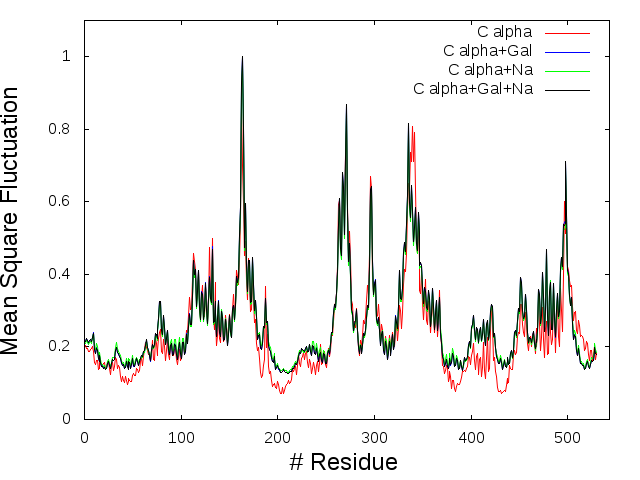
\includegraphics[scale=0.35]{./Kap4/ANM/ANM_server/grafica_11_A_n.png}
    \put(-28,-4){(a)$R_c=11\AA$}
      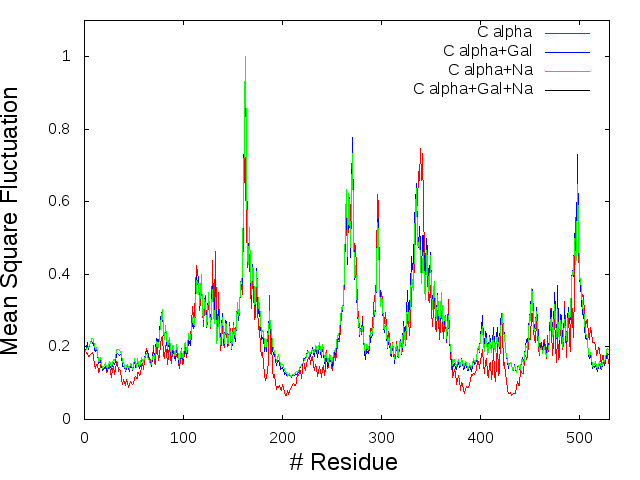
\includegraphics[scale=0.35]{./Kap4/ANM/ANM_server/grafica_12_A_n.png}
     \put(-28,-4){(a)$R_c=12\AA$}
\caption{Fluctuaciones ms normalizadas en funci\'{o}n del n\'{u}mero de residuo para $ R_c=11\AA$ y $R_c= 12\AA$ usando  los primeros 100 modos. Los diferentes colores indican si la simulaci\'{o}n fue realizada sin el ion, el sustrato, con alguno de ellos o ambos.}\label{fig:ANM_pre3}
\end{figure}
Los segmentos que cambian antes y despu\'{e}s de entrar el \ce{Na^{+}} son TM3, TM7, TM8, la regi\'{o}n desordenada entre TM9 y TM10, TM11 y la regi\'{o}n entre TM12 y TM13. Tambi\'{e}n cambia TM14. De estos uno de los menos relevantes es el segmento TM14. Los otros han sido encontrados con las anteriores distancias de corte.\\

Entre TM12 y TM13, hay un lazo $\omega$ que une a los dos segmentos, este se encuentra en el espacio intracelular, por eso, tiene tanta libertad de moverse y pueden detectarse f\'{a}cilmente los cambios que ocurren en el co-transportador cuando se le a\~{n}ade una especie qu\'{i}mica.Al igual que en el caso de $10\AA$ se encuentra que las fluctuaciones ms aumentan cuando se a\~{n}ade el sodio. Luego, cuando se encuentran unidos tanto el sodio como la galactosa, las fluctuaciones en esa regi\'{o}n disminuyen, debido posiblemente al aumento de restricciones que impone la galactosa, como tambi\'{e}n puede deberse a la entrega de energ\'{i}a del cotransportador a la galactosa. Aunque este sitio no est\'{a} en el sitio activo, ser\'{i}a interesante poder medir experimentalmente las diferencias en los movimientos en las regiones desordenadas alejadas de la prote\'{i}na ya que estas son m\'{a}s flexibles y por tanto m\'{a}s sensibles a los cambios.\\
\subsubsection{Distancias de corte $R_c=13\AA$ y $R_c= 14\AA$}
A simple vista las fluctuaciones ms para los carbonos $\alpha$ y los carbonos $\alpha$ con el \ce{Na^{+}} (gr\'{a}fica roja) y la galactosa (gr\'{a}fica negra) difieren poco, igualmente ocurre al comparar el caso en que est\'{a} unido \'{u}nicamente el \ce{Na^{+}} (verde) con el caso en que est\'{a} unida la galactosa (azul).\\

Las regiones con las menores fluctuaciones nuevamente est\'{a}n alrededor de Ile253 (TM7), Phe479 (entre TM12 y TM13) y Glu88 (TM3). Se observa que en los segmentos TM3 y TM7 se ve un cambio menor entre cada uno de los estados del cotransportador comparado con las distancias de corte $R_c=11\AA$ y $R_c=12\AA$. Pero contrario a estas distancias de corte, cuando la galactosa y el \ce{Na^{+}} est\'{a}n unidos, las fluctuaciones ms son menores que cuando el cotransportador est\'{a} solo.\\
La secuencia de los movimientos de los segmentos TM3 y TM7 ser\'{i}a la siguiente: El cotransportador est\'{a} solo (gr\'{a}fica roja), se une el \ce{Na^{+}} y se vuelve m\'{a}s flexible (gr\'{a}fica verde), al complejo cotransportador+\ce{Na^{+}} se une la galactosa y se vuelve menos flexible que lo que era originalmente (gr\'{a}fica  negra).
\begin{figure}[h]
 \centering
       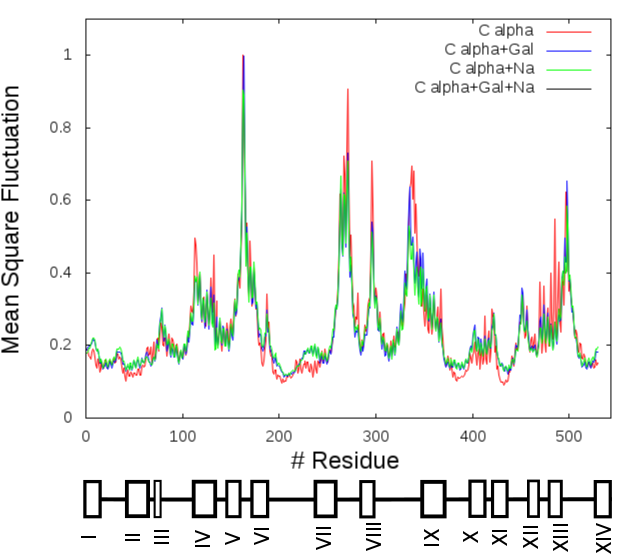
\includegraphics[scale=0.35]{./Kap4/ANM/ANM_server/grafica_13_A_n.png}
     \put(-28,-4){(a)$R_c=13\AA$}
       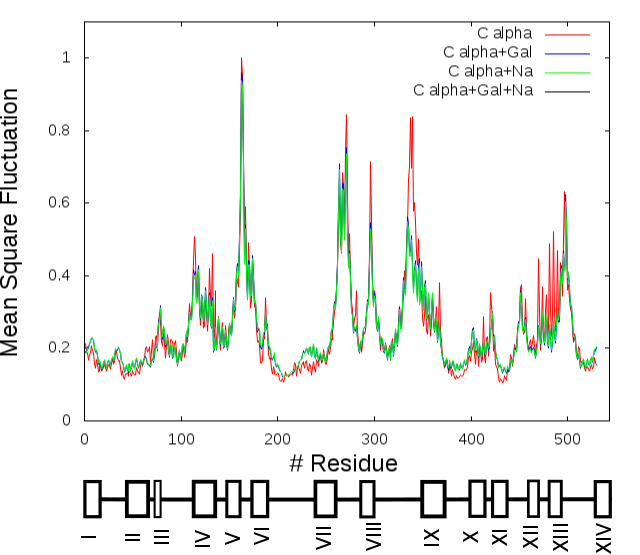
\includegraphics[scale=0.35]{./Kap4/ANM/ANM_server/grafica_14_A_n.png}
\put(-28,-4){(a)$R_c=14\AA$}
\caption{Fluctuaciones ms normalizadas en funci\'{o}n del n\'{u}mero de residuo para $ R_c=13\AA$ y $R_c= 14\AA$ usando  los primeros 100 modos. Los diferentes colores indican si la simulaci\'{o}n fue realizada sin el ion, el sustrato, con alguno de ellos o ambos.}\label{fig:ANM_pre4}
\end{figure}
%\newpage
\section{ANM de vSGLT con la Estructura Completa}
\subsection{Preparaci\'{o}n del PDB}
Ya que en el mutante de vSGLT en la posici\'{o}n K294A, llamado 2XQ2 aparece resuelta la estructura cristalina del TM1 perteneciente a la cadena A, se usa el programa PyMol, y como archivos de entrada los pdbs 3DH4 y el de su mutante 2XQ2, para crear un archivo que sea cercano a la estructura real objeto de estudio, esto es, al cotransportador vSGLT. Se a\~{n}ade a 3DH4 la h\'{e}lice 1 resuelta, tal como aparece en la figura \ref{fig:vSGLT_in_2}.\\
\begin{figure}[h]
 \centering
 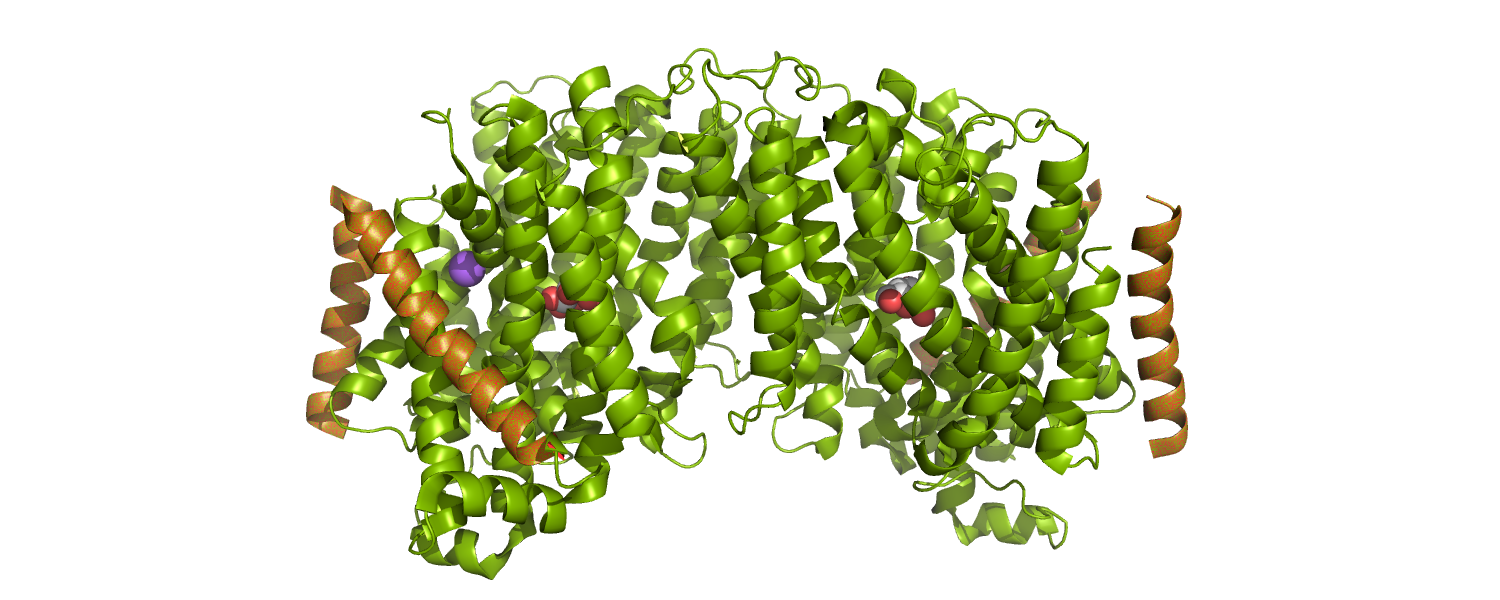
\includegraphics[scale=0.3]{Kap4/vSGLT_n.png}
 % vSGLT_n.png: 0x0 pixel, 300dpi, 0.00x0.00 cm, bb=
 \caption{Estructura del cotransportador vSGLT en su conformaci\'{o}n ocluida junto con las h\'{e}lices 1 y 15 a\~{n}adidas mediante PyMol.}
 \label{fig:vSGLT_in_2}
\end{figure}
\subsection{Metodolog\'{i}a}
Mediante el servidor ANM, se ha realizado un estudio del simportador vSGLT en la conformaci\'{o}n hacia adentro y a\~{n}adiendo las nuevas h\'{e}lices encontradas (color marr\'{o}n figura \ref{fig:vSGLT_in_2}), el pdb obtenido con PyMol tiene forma de d\'{i}mero, como aparece biol\'{o}gicamente. \\

Una vez ingresado el archivo pdb se selecciona el modelo de la estructura. Inicialmente se toman s\'{o}lamente los carbonos $\alpha$ del co-transportador, se seleccionan las distancias de corte $R_c$ entre $7\AA$ y $20\AA$. Adem\'{a}s, el factor de peso aplicado a las distancias de corte es $s=0$, es decir, las distancias de corte en el hessiano \eqref{eq:hes} son fijas \cite{Zimmermann2011}. Luego se calculan los modos normales $(\lambda_k,a_k)$ (autovalores, autovectores) y los factores b mediante la parte del c\'{o}digo escrita en Fortran. Se hace otro NMA agregando los \'{a}tomos de la galactosa (sin hidr\'{o}genos), agregando el sodio y luego agregando tanto el ion como el sustrato.\\
\subsection{Resultados}
En la figuras% \label{fig:ANM_pos}
\ref{fig:ANM_pos1}, \ref{fig:ANM_pos2} y \ref{fig:ANM_pos3} %y \ref{fig:ANM_pos4}
se muestran los factores b por cada n\'{u}mero de residuo (entre 9 y 560) y para cada distancia de corte $R_c$, entre $8\AA$ y $20\AA$ \footnote{S\'{o}lamente se muestran las distancias de corte $R_c=9\AA$, $R_c=12\AA$ y $R_c=18\AA$ debido a que el resultado de $R_c=8\AA$ es similar al de $R_c=9\AA$, los resultados desde $R_c=10\AA$ hasta $R_c=16\AA$ son similares a los de $R_c=12\AA$ y los resultados desde $R_c=17\AA$ hasta $R_c=20\AA$ son similares a los de $R_c=18\AA$} de la cadena A. Ha de notarse que al igual que el ANM previo, para distancias de corte menores o iguales a $7\AA$,no se encontraron todos  los autovalores, ni autovectores, ni factores b, ya que no todos los autovalores convergen \cite{Zimmermann2011}.\\

En las tres gr\'{a}ficas se observa que la adici\'{o}n de las $\alpha$ h\'{e}lices genera una disminuci\'{o}n en los cambios de los movimientos globales, esto debido a que una $\alpha$ h\'{e}lice es una estructura estable y r\'{i}gida, comparada con las regiones desordenadas y con las hojas $\beta$. Este resultado es acorde con los resultados presentados en \cite{Adelman2016}, en donde al incluir las $\alpha$ h\'{e}lices resueltas, hay una mayor estabilidad del cotransportador en presencia del ion.\\

De acuerdo a la tabla \ref{tab:flu4} del anexo \ref{AnexoB}, en todos los casos se encuentran picos que corresponden a las regiones entre los residuos Ala47 y Gly48\footnote{Ya que a\'{u}n son desconocidas las posiciones de los residuos entre 29 y 47 se le suma 17 a cada valor de la tabla. Ejemplo: $30+17=47$, $31+17=48$, $301+17=318$, $526+17=542$ y as\'{i} a partir del residuo 29}, Met318, Phe542 y Gly556.\\
 \begin{figure}[h]
  \centering
     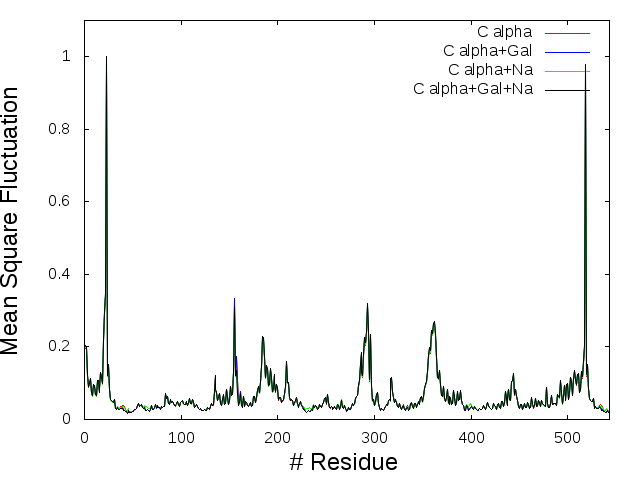
\includegraphics[scale=0.25]{./Kap4/ANM/ANM_s_nuevo/grafica_9_A_n.png}
    \put(-28,-4){$R_c=9\AA$}
 \caption{Fluctuaciones ms normalizadas en funci\'{o}n del n\'{u}mero de residuo para $R_c=9\AA$ usando  los primeros 100 modos. Los diferentes colores indican si la simulaci\'{o}n fue realizada sin el ion, el sustrato, con alguno de ellos o ambos.}\label{fig:ANM_pos1}
 \end{figure}
 Ala47 y Gly48 est\'{a}n justo antes del segmento TM2 en una regi\'{o}n desordenada del periplasma. Sus altas fluctuaciones para $R_c=9\AA$ son naturales debido a que de acuerdo al modelo no aparecen conectados los segmentos TM1 y TM2. Sin embargo, al aumentar la distancia de corte las fluctuaciones ms de este pico disminuyen como consecuencia del aumento en el n\'{u}mero de restricciones de estos residuos.\\
 \begin{figure}[h]
  \centering
       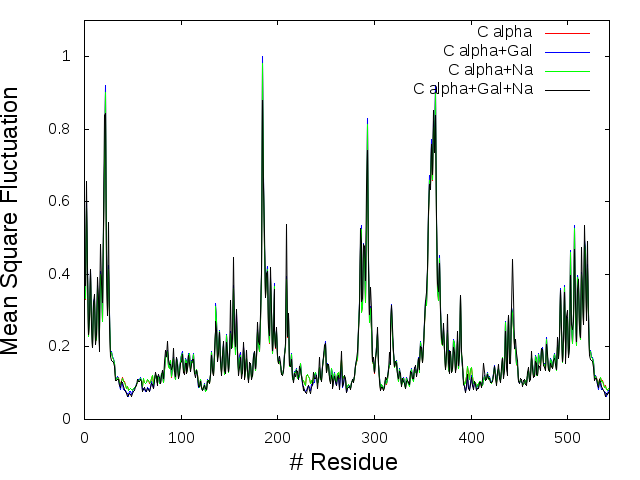
\includegraphics[scale=0.25]{./Kap4/ANM/ANM_s_nuevo/grafica_12_A_n.png}
      \put(-28,-4){$R_c=12\AA$}
 \caption{Fluctuaciones ms normalizadas en funci\'{o}n del n\'{u}mero de residuo para $R_c=12\AA$ usando  los primeros 100 modos. Los diferentes colores indican si la simulaci\'{o}n fue realizada sin el ion, el sustrato, con alguno de ellos o ambos.}\label{fig:ANM_pos2}
 \end{figure}
  
 El residuo Met318 est\'{a} en una peque\~{n}a $\alpha$ h\'{e}lice que une los segmentos TM8 y TM9. Esta peque\~{n}a $\alpha$ h\'{e}lice se encuentra en el citoplasma, por eso es m\'{a}s flexible. Sorpresivamente se encuentra que a medida que aumenta la distancia de corte, esta regi\'{o}n aumenta sus fluctuaciones, volvi\'{e}ndose m\'{a}s flexible.\\
 El residuo Phe542 est\'{a} en el segmento TM14 que se encuentra dentro del citoplasma, como se mencion\'{o} en el ANM previo, ver figura \ref{fig:W543}. Como TM4 no se conecta con sus residuos a distancias de corte bajas es m\'{a}s flexible que cuando se incrementa la distancia de corte.\\
 
 Para $R_c=12\AA$ se detecta un m\'{i}nimo con cambios alrededor del residuo Gln69 (En la gr\'{a}fica residuo 52) que se encuentra dentro del segmento TM2, este segmento es el que act\'{u}a como bolsillo para el sodio y la galactosa. En efecto, la glutamina interact\'{u}a con la galactosa ya que es un residuo polar descargado. Por otro lado, los residuos mostrados en forma de varillas en la figura \ref{fig:Na_Gal} est\'{a}n conectados a $R_c=12\AA$ con el sodio. Cuando el cotransportador est\'{a} solo o tiene el sodio no hay diferencias significativas, pero cuando se unen tanto el sodio como la galactosa las fluctuaciones ms disminuyen.\\ 
 \begin{figure}[h]
  \centering
     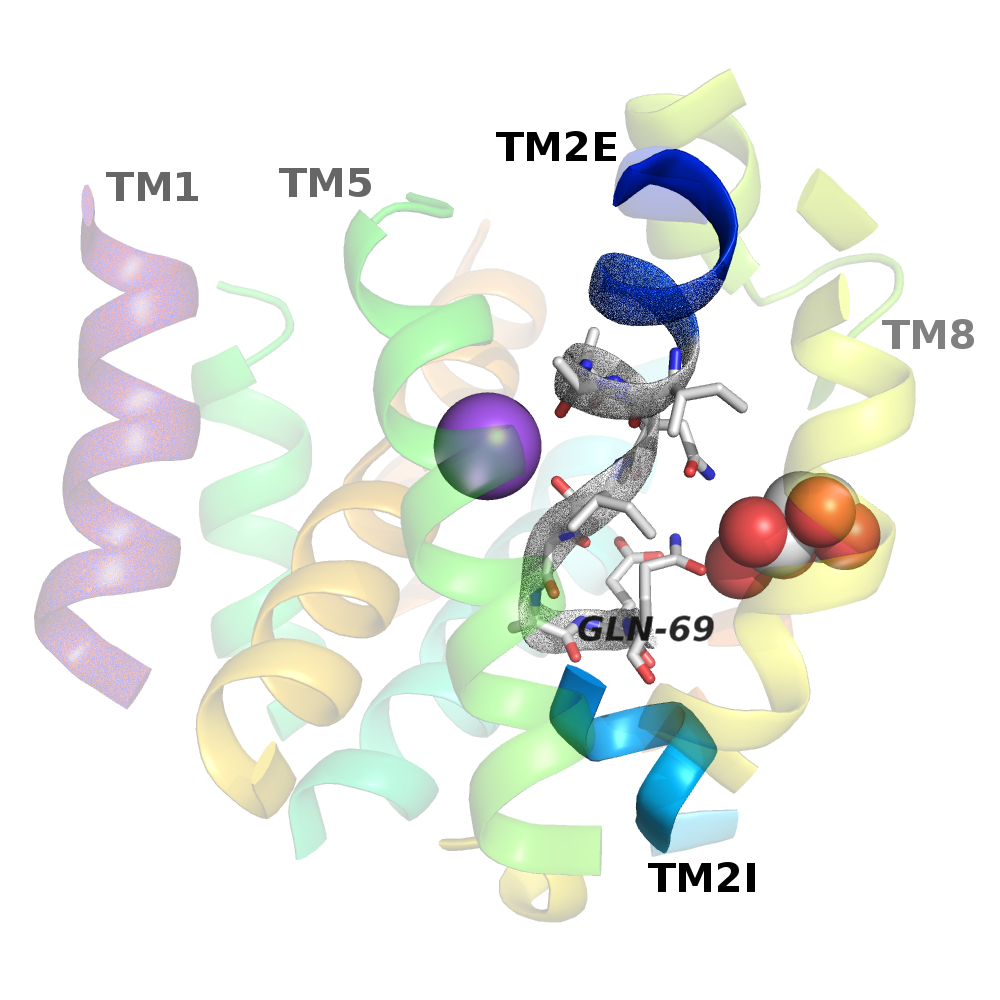
\includegraphics[scale=0.1]{./Kap4/h2_label.png}
 \caption{Contactos entre el \ce{Na^{+}}, la galactosa y el segmento TM2.}\label{fig:Na_Gal}
 \end{figure}
 \begin{figure}[h]
  \centering
     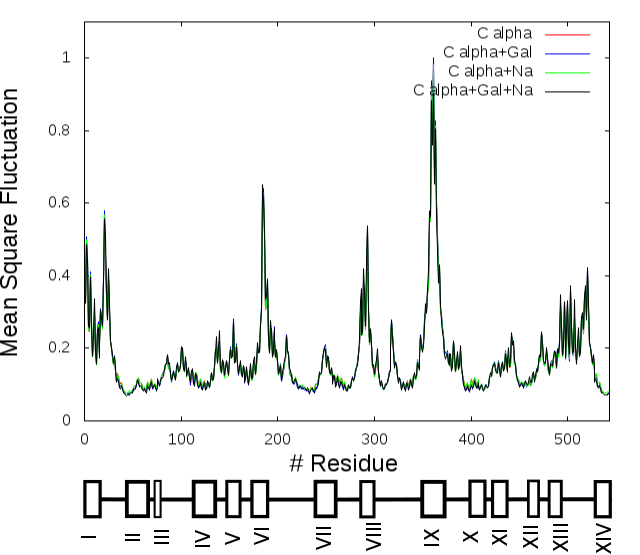
\includegraphics[scale=0.25]{./Kap4/ANM/ANM_s_nuevo/grafica_18_A_n.png}
    \put(-28,-4){$R_c=18\AA$}
 \caption{Fluctuaciones ms normalizadas en funci\'{o}n del n\'{u}mero de residuo para $R_c=18\AA$ usando  los primeros 100 modos. Los diferentes colores indican si la simulaci\'{o}n fue realizada sin el ion, el sustrato, con alguno de ellos o ambos.}\label{fig:ANM_pos3}
 \end{figure}
 
 %\begin{figure}[h]
%\centering
%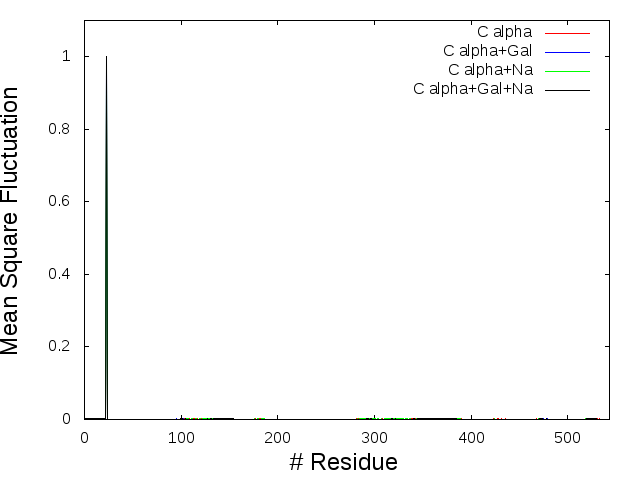
\includegraphics[scale=0.2]{./Kap4/ANM/ANM_s_nuevo/grafica_7_A_n.png}
 %  \put(-50,-2){$R_c=7\AA$}
% %  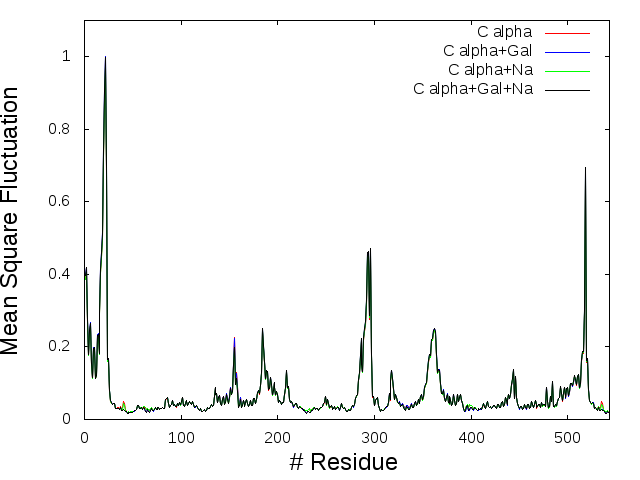
\includegraphics[scale=0.2]{./Kap4/ANM/ANM_s_nuevo/grafica_8_A_n.png}
%   \put(-50,-2){$R_c=8\AA$}
%   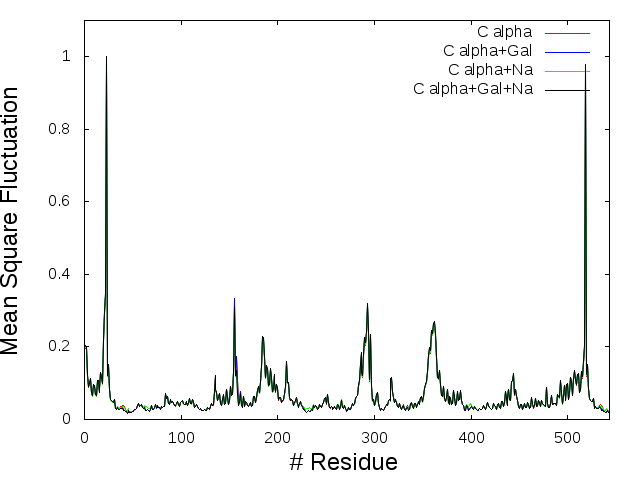
\includegraphics[scale=0.2]{./Kap4/ANM/ANM_s_nuevo/grafica_9_A_n.png}
%   \put(-50,-2){$R_c=9\AA$}
%    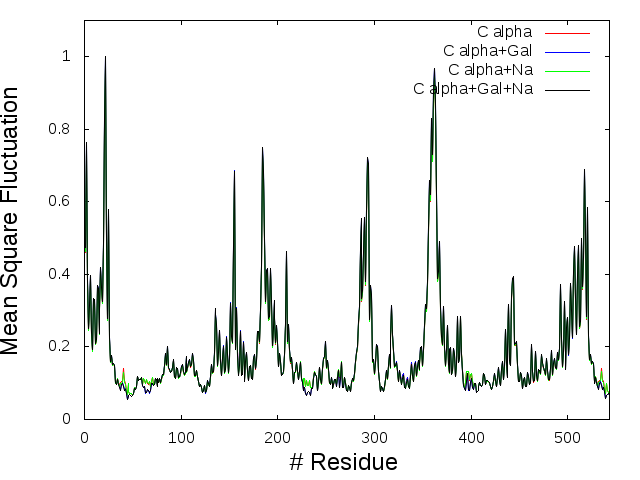
\includegraphics[scale=0.2]{./Kap4/ANM/ANM_s_nuevo/grafica_10_A_n.png}
%    \put(-50,-2){$R_c=10\AA$}
%   \vspace{1mm}
%     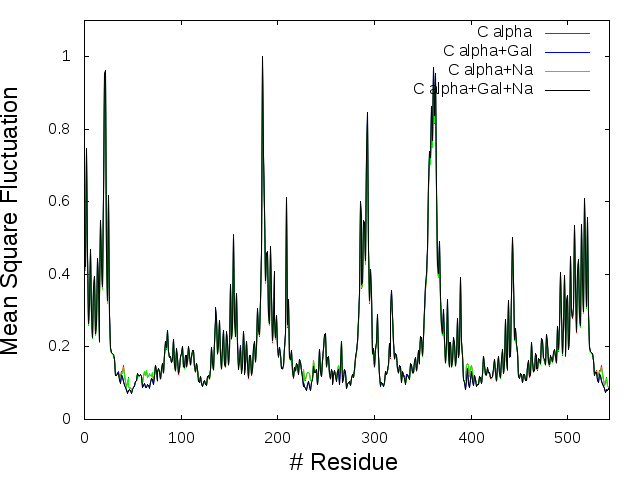
\includegraphics[scale=0.2]{./Kap4/ANM/ANM_s_nuevo/grafica_11_A_n.png}
%     \put(-50,-2){$R_c=11\AA$}
%      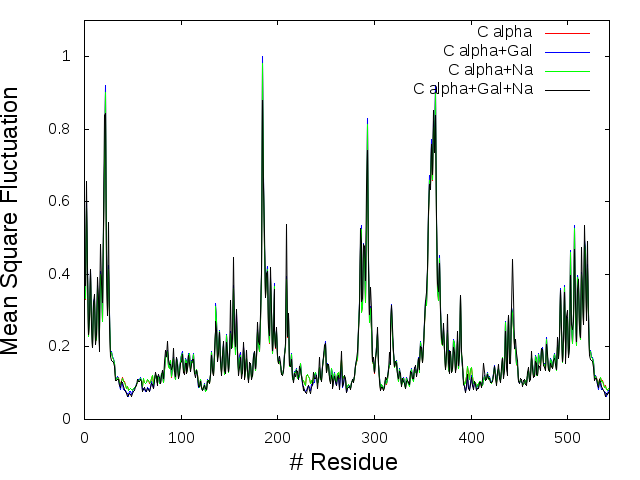
\includegraphics[scale=0.2]{./Kap4/ANM/ANM_s_nuevo/grafica_12_A_n.png}
%     \put(-50,-2){$R_c=12\AA$}
%       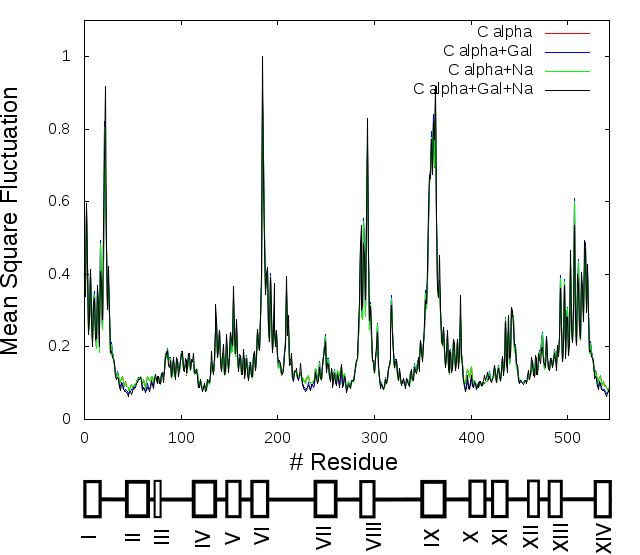
\includegraphics[scale=0.2]{./Kap4/ANM/ANM_s_nuevo/grafica_13_A_n.png}
%       \put(-50,-2){$R_c=13\AA$}
%     \vspace{1mm}
%       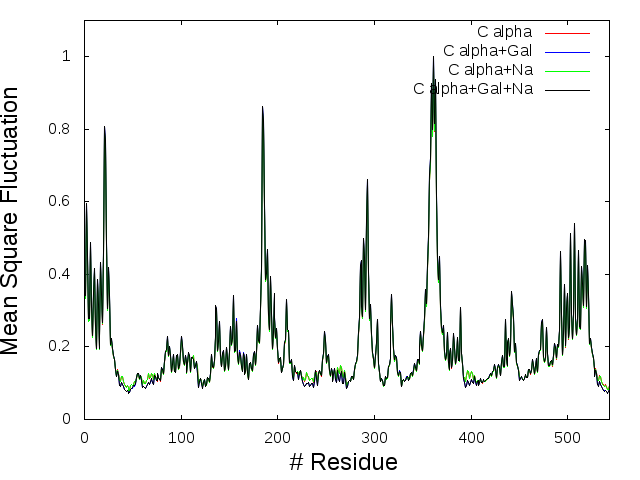
\includegraphics[scale=0.2]{./Kap4/ANM/ANM_s_nuevo/grafica_14_A_n.png}
% \put(-50,-2){$R_c=14\AA$}
%       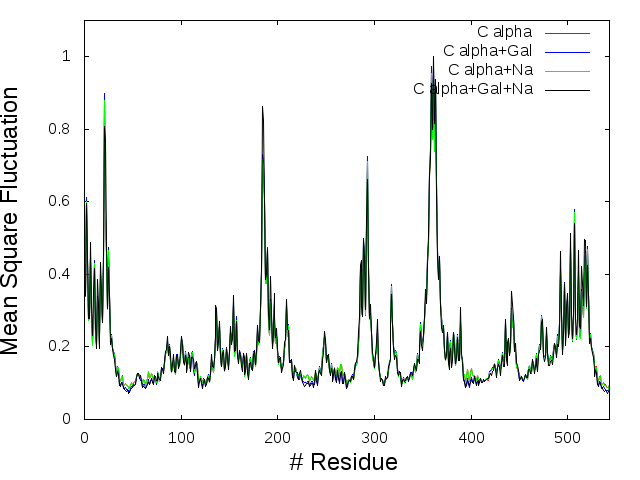
\includegraphics[scale=0.2]{./Kap4/ANM/ANM_s_nuevo/grafica_15_A_n.png}
% \put(-50,-2){$R_c=15\AA$}
%       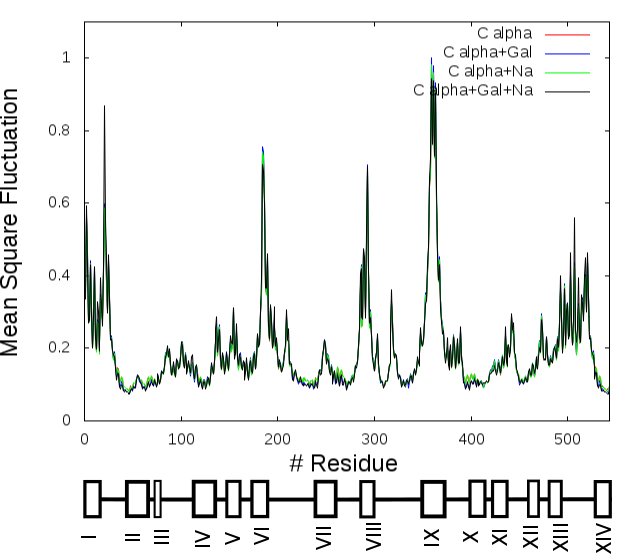
\includegraphics[scale=0.2]{./Kap4/ANM/ANM_s_nuevo/grafica_16_A_n.png}
% \put(-50,-2){$R_c=16\AA$}
% \vspace{1mm}
%        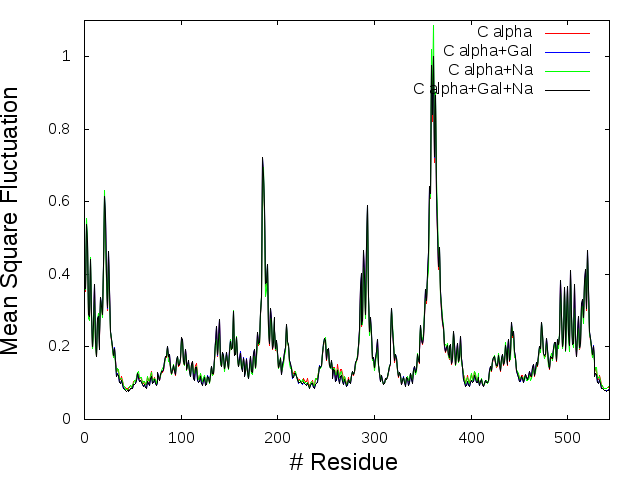
\includegraphics[scale=0.2]{./Kap4/ANM/ANM_s_nuevo/grafica_17_A_n.png}
% \put(-50,-2){$R_c=17\AA$}
%       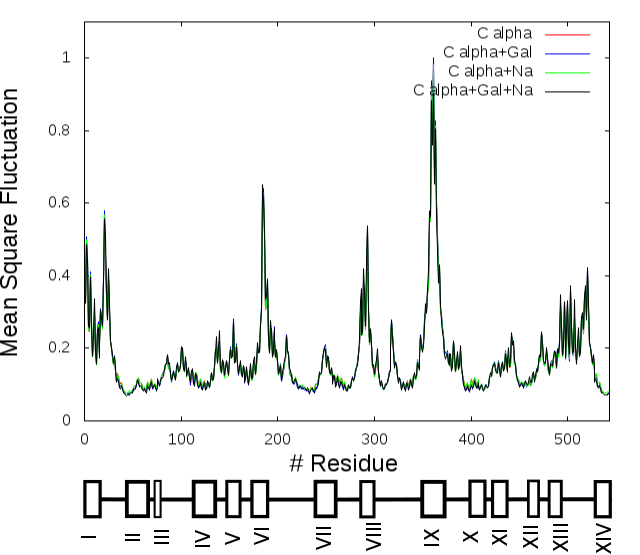
\includegraphics[scale=0.2]{./Kap4/ANM/ANM_s_nuevo/grafica_18_A_n.png}
% \put(-50,-2){$R_c=18\AA$}
%       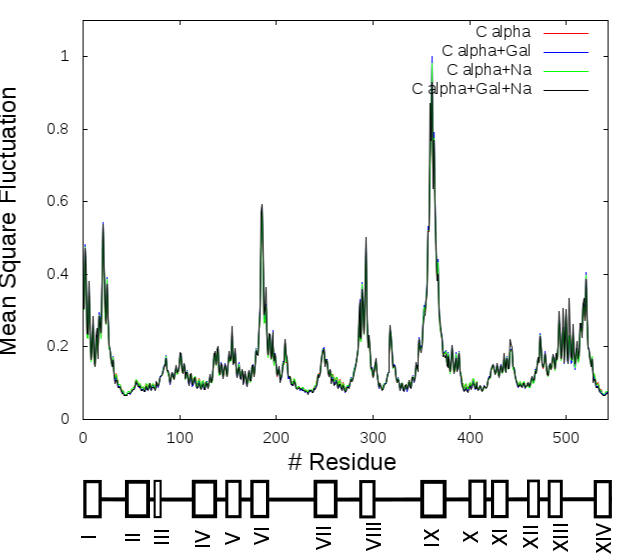
\includegraphics[scale=0.2]{./Kap4/ANM/ANM_s_nuevo/grafica_19_A_n.png}
% \put(-50,-2){$R_c=19\AA$}
% \vspace{1mm}
%       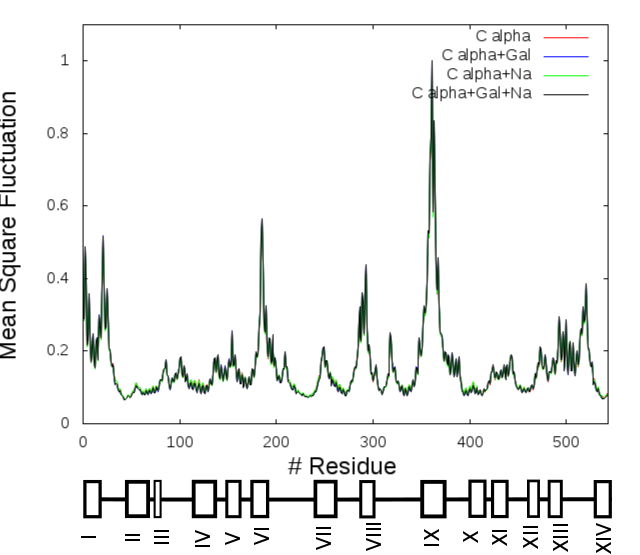
\includegraphics[scale=0.2]{./Kap4/ANM/ANM_s_nuevo/grafica_20_A_n.png}
% \put(-50,-2){$R_c=20\AA$}
%  \caption{Fluctuaciones ms normalizadas en funci\'{o}n del n\'{u}mero de residuo entre $8\AA\leq R_c\leq 20\AA$ usando  los primeros 100 modos. Los diferentes colores indican si la simulaci\'{o}n fue realizada sin el ion, el sustrato, con alguno de ellos o ambos.}\label{fig:ANM_pos}
% \end{figure}
